\documentclass[10pt,a4paper]{article}
\usepackage[margin=2cm]{geometry}
\usepackage{amsmath,amssymb,booktabs,graphicx,caption,subcaption,xcolor,float,hyperref,tikz}
\usetikzlibrary{arrows.meta,positioning,fit,calc}
\hypersetup{colorlinks=true,linkcolor=blue!50!black,urlcolor=blue!50!black}
\captionsetup{font=small,labelfont=bf}
\newcounter{diagram}
\newcommand{\diagramcaption}[1]{\refstepcounter{diagram}\par\smallskip\noindent{\small\textbf{Diagram~\thediagram.} #1}}
\title{\vspace{-1.2cm}\textbf{A swarm that owns a proof can still lose it}\\[2pt]
\large Simulation 1 (days and nights), setup \texttt{task003-symmetric}}
\author{LLM-free simulator; report of 14 October 2026; runs of 7 October 2026\\
\small Mirrors the Simulation 2 report on \texttt{task003-symmetric} of the same date, section by section.}
\date{}
\begin{document}
\maketitle
\vspace{-1cm}

\paragraph{How the simulator works.} The world, \texttt{task\_003}, has three candidate
allocations; A0 is the correct one. Each of 24 agents is given one true fact about it and reasons as
an exact Bayesian: its \emph{belief} is the exact probability of A0, A1 and A2 given the facts it
currently remembers. An episode has 30 rounds, each a day and a night. During the day the agents act
one at a time in a new random order: an agent reads $q$ posts drawn at random from a shared
\emph{board} (never its own), adds their facts to its memory, recomputes its belief, \emph{votes}
(\emph{argmax}: the most probable allocation; \emph{probability matching}: a vote drawn from its
belief) and posts one remembered fact that supports its vote, or nothing if none does. At night a
\emph{controller} with a target, A0 (truth) or A2 (false), reads $q_c$ agent posts; unless at least
75\% of them come from agents voting for its target, or what it read already proves its target, it
posts the $b$ facts from its own pool that best support its target. The board is then cleared,
keeping only the controller's new posts. At each dawn every remembered fact is forgotten with
probability $1-\rho$ and comes back if read again. Every episode is run three times with the same
random draws: without a controller, with the truth controller and with the false controller.

\paragraph{Summary.} 24 agents together hold a complete proof that allocation A0 is
correct, but no single agent does. A controller steers toward A0 (truth) or A2
(false). Agents vote by probability matching, as in Simulation 2; other agent rules are in
Section~\ref{sec:rules}. (i)~\textbf{Whether the false controller wins depends on memory}: when
agents forget it pulls a large part of the swarm to A2; with full memory its success is temporary,
because its own true facts end up completing proofs of A0. (ii)~\textbf{The false controller is
stronger than in Simulation 2} ($0.22$ against $0.11$ in votes, one fact per night), and a larger
posting budget makes it stronger still. (iii)~\textbf{The controller senses the swarm accurately}, so
its failures are not sensing failures. (iv)~\textbf{Helping the truth is not the same as helping
agents assemble their own proof}. (v)~Measured by the swarm's \emph{collective decision},
\textbf{overturning the proof has increasing returns}: concentrating control in some runs beats every
tested setting.

\section{Setup}

\begin{center}
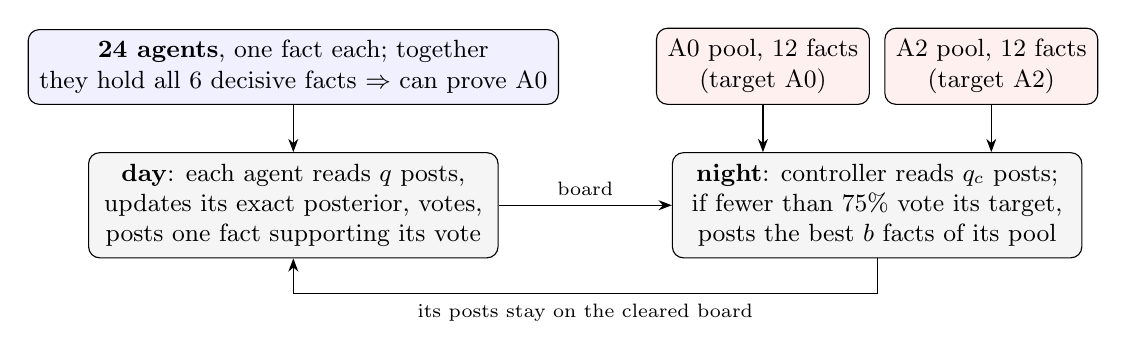
\begin{tikzpicture}[font=\small, box/.style={draw, rounded corners, align=center, inner sep=4pt}]
  \node[box, fill=gray!8, minimum width=5.2cm] (day) {\textbf{day}: each agent reads $q$ posts,\\
     updates its exact posterior, votes,\\ posts one fact supporting its vote};
  \node[box, fill=gray!8, right=2.2cm of day, minimum width=5.2cm] (night) {\textbf{night}: controller reads $q_c$ posts;\\
     if fewer than 75\% vote its target,\\ posts the best $b$ facts of its pool};
  \node[box, fill=blue!6, above=0.6cm of day, minimum width=5.2cm] (agents) {\textbf{24 agents}, one fact each; together\\
     they hold all 6 decisive facts $\Rightarrow$ can prove A0};
  \node[box, fill=red!6, above=0.6cm of night, xshift=-1.45cm] (p0) {A0 pool, 12 facts\\ (target A0)};
  \node[box, fill=red!6, above=0.6cm of night, xshift=1.45cm] (p2) {A2 pool, 12 facts\\ (target A2)};
  \draw[-{Stealth}] (agents) -- (day);
  \draw[-{Stealth}] (p0) -- (p0 |- night.north);
  \draw[-{Stealth}] (p2) -- (p2 |- night.north);
  \draw[-{Stealth}] (day) -- node[above, font=\scriptsize]{board} (night);
  \draw[-{Stealth}] (night.south) -- ++(0,-0.45) -| node[below, pos=0.25, font=\scriptsize]{its posts stay on the cleared board} (day.south);
\end{tikzpicture}
\diagramcaption{One round of Simulation 1: a day followed by a night, repeated for 30
rounds. Each dawn, every remembered fact survives with probability $\rho$.}
\label{dia:setup}
\end{center}

The two pools share no fact, contain no decisive fact, cannot prove their target, and
are matched in strength pair by pair. Agents are exact Bayesian reasoners: an agent's belief is the
exact posterior over the three allocations given the facts it remembers. Every episode is run three
times with the same random draws: silent, truth controller, false controller. The \emph{paired
gain} of a controller in the share of agents voting for allocation $a$ on day $t$ is
\begin{equation}\label{eq:gain}
G_t^{(a)} = \frac{1}{E}\sum_{e=1}^{E}\Bigl[x_{a,t}^{\text{ctrl}}(e) - x_{a,t}^{\text{silent}}(e)\Bigr],
\end{equation}
with $E = 1000$ episodes per cell and 95\% intervals from resampling episodes. (Simulation 2 measures
the gain in mean \emph{belief}; Table~\ref{tab:gain} also gives its gain in votes, and
Figure~\ref{fig:votes} shows the vote shares of both simulations on the same scale.) The grid:
$q \in \{3,6,12\}$, $q_c \in \{3,6,12,24\}$, $b \in \{1,2,3,6,9\}$, $\rho \in \{0.75, 1\}$. Unless
stated otherwise: probability matching, $q = 6$, $q_c = 12$, $b = 3$.

\section{Main result: the false controller can pull the swarm off its proof only when agents forget}

\begin{figure}[H]
\centering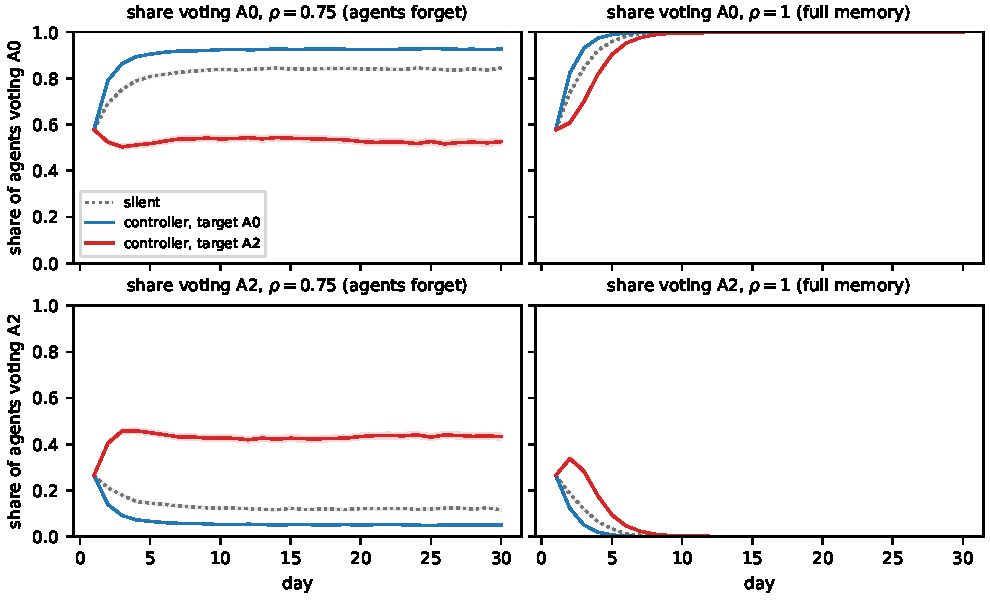
\includegraphics[width=0.84\linewidth]{figures/fig_votes_time.pdf}
\caption{Share of the 24 agents voting A0 (top) and A2 (bottom) at the end of each day, without a
controller (dotted grey), with the controller targeting A0 (blue) and with the one targeting A2 (red);
$\rho = 0.75$ (left) and $\rho = 1$ (right). Bands: 95\% intervals. Probability matching, $q = 6$,
$q_c = 12$, $b = 3$.}
\label{fig:votes}
\end{figure}

\begin{itemize}\itemsep1pt
\item \textbf{Without a controller the swarm backs the truth}: on day 30, 85\% vote A0 and 12\% A2
  when agents forget; with full memory every agent votes A0 from about day 8.
\item \textbf{When agents forget, the false controller pulls a large part of the swarm away}: the A2
  share more than triples (0.43 against 0.12) and the A0 share falls to 0.53; the truth controller
  raises A0 to 0.93.
\item \textbf{With full memory the false controller wins only briefly}: an early bump in A2 (0.34 on
  day 2), then every agent votes A0.
\end{itemize}

\paragraph{Without a controller, compared with Simulation 2.} In votes the silent swarms of the two
simulations agree: on day 30, 85\% vote A0 at $q = 6$ (Simulation 2: 85\%) and 94\% at $q = 12$ (94\%).
Here the day-end snapshot comes before dawn's forgetting, so beliefs and votes agree; in Simulation 2 a
snapshot at a fixed time catches faded memories and shows lower beliefs. More agents hold a complete
proof here (28\% against 12\% at $q = 6$); how much of that gap is the timing of the snapshot has not
been separated.

\begin{table}[H]
\centering\small
\caption{Day-30 paired gain in the target's vote share, Eq.~(\ref{eq:gain}), $\rho = 0.75$, $q_c = 12$,
for $q = 3 / 6 / 12$; probability matching. Simulation 2: $\lambda_c = 1$ (about one fact per time
unit), gate on, same $q$, $q_c$. With full memory every gain is 0.}
\label{tab:gain}
\begin{tabular}{lccc}
\toprule
controller & Simulation 1, $b = 1$ & Simulation 1, $b = 3$ & Simulation 2, votes \\
\midrule
truth (A0) & 0.17 / 0.08 / 0.01 & 0.17 / 0.08 / 0.02 & 0.14 / 0.08 / 0.04 \\
false (A2) & 0.41 / 0.22 / 0.06 & 0.48 / 0.32 / 0.08 & 0.24 / 0.11 / 0.04 \\
\bottomrule
\end{tabular}
\end{table}

\begin{figure}[H]
\centering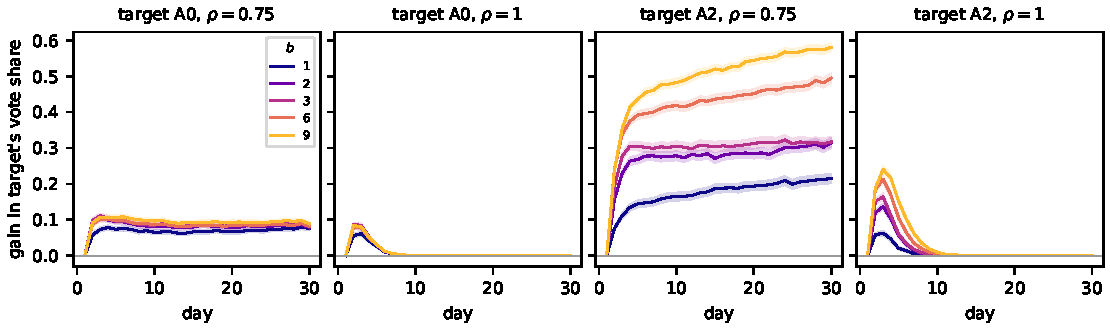
\includegraphics[width=0.98\linewidth]{figures/fig_gain_time.pdf}
\caption{Paired gain in the target's vote share over the days, Eq.~(\ref{eq:gain}), one line per
posting budget $b$. Bands: 95\% intervals.}
\label{fig:gaintime}
\end{figure}

\begin{figure}[H]
\centering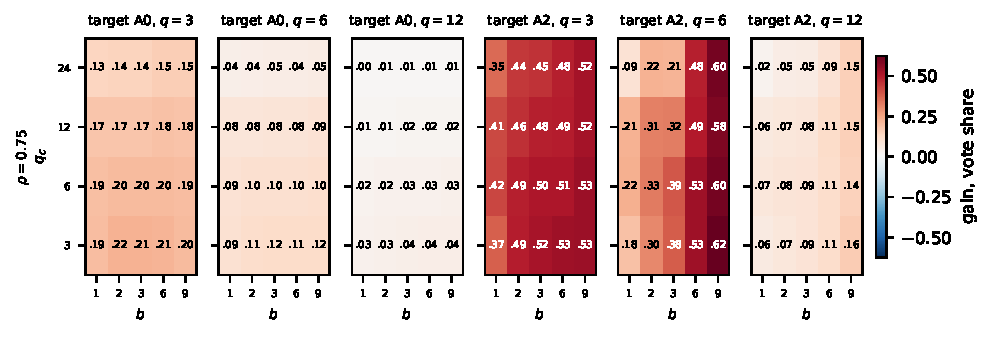
\includegraphics[width=0.98\linewidth]{figures/fig_phase_gain.pdf}
\caption{Day-30 paired gain over the facts per night $b$ (x) and the posts the controller reads
$q_c$ (y), for each target and every $q$ (columns), $\rho = 0.75$; probability matching. With full
memory every gain is 0. Grey number: the 95\% interval includes 0.}
\label{fig:phase}
\end{figure}

\begin{itemize}\itemsep1pt
\item \textbf{The false controller is stronger than in Simulation 2}: with about one fact per time
  unit, $0.22$ against $0.11$ in votes at $q = 6$ (Table~\ref{tab:gain}). The truth controller is the
  same ($0.08$ in both).
\item \textbf{Reading more defends the proof}: the false controller's gain falls from $0.48$ at $q = 3$
  to $0.08$ at $q = 12$ ($b = 3$). Agents who hold pieces of the proof keep posting them, so readers
  keep meeting them.
\item \textbf{The gain is reached within a few days and then stays} (Figure~\ref{fig:gaintime}); with
  full memory it returns to 0 within about ten days.
\end{itemize}

\section{The controller's strength, the vote gate and the proof stop}\label{sec:strength}

\subsection{Strength: the posting budget}

\begin{figure}[H]
\centering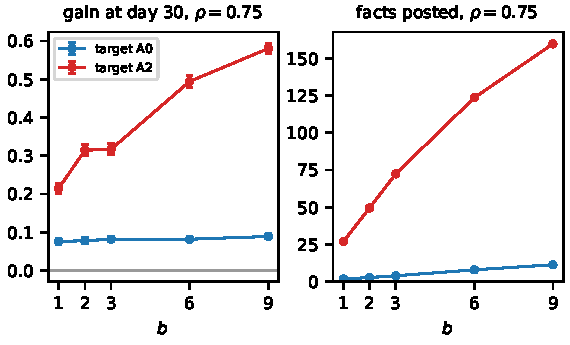
\includegraphics[width=0.5\linewidth]{figures/fig_strength.pdf}
\caption{Day-30 gain and facts posted (mean per episode, over 30 nights) against the facts per night
$b$ (target A0 blue, A2 red); $\rho = 0.75$, $q = 6$, $q_c = 12$. Bars: 95\% intervals.}
\label{fig:strength}
\end{figure}

\begin{itemize}\itemsep1pt
\item \textbf{A larger posting budget helps the false controller}: its gain grows from $0.22$ at
  $b = 1$ to $0.58$ at $b = 9$, while the facts it posts grow from about 27 to 166 per episode.
  Each pool lies entirely on its target's side, so more posts mean more evidence for A2 (unlike in
  \texttt{task003-nosolution}, where a large budget backfires).
\item \textbf{The truth controller's gain stays at 0.08--0.09}: the silent swarm already sits near
  85\% A0, so the vote gate keeps it silent on most nights.
\end{itemize}

\subsection{The vote gate and the proof stop}

Simulation 1 has no gate-off arm: the controller is always silent when at least 75\% of the posts it
reads come from agents voting for its target. The false controller is rarely stopped (the A2 share
rarely reaches 75\%); the truth controller often is. The proof stop (silent when what it read already
proves its target) was switched off in a separate run for the truth controller: it fires on about 30\%
of nights, but with it off the controller posts on at most 2\% of nights, because the gate already
silences it (Table~\ref{tab:rule}).

\section{Who holds the proof}\label{sec:proof}

\begin{figure}[H]
\centering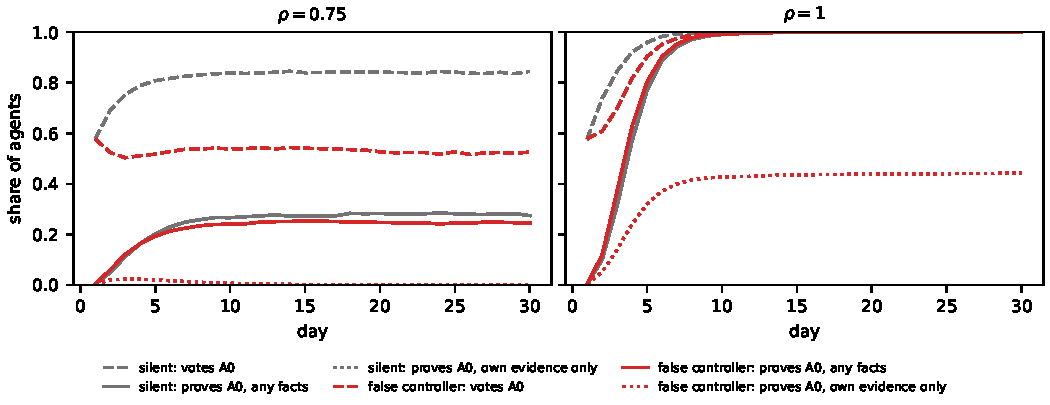
\includegraphics[width=0.95\linewidth]{figures/fig_proof_time.pdf}
\caption{Share of agents voting A0 (dashed), holding a proof of A0 from any facts they remember
(solid) and from their own original evidence only (dotted); silent (grey) against the false
controller (red). Probability matching, $q = 6$, $q_c = 12$, $b = 3$.}
\label{fig:proof}
\end{figure}

\paragraph{Why memory decides.} With forgetting, a proof must be reassembled continually: on day 30,
28\% of silent agents hold one, all from the agents' own facts. Under the false controller about as
many hold a proof (25\%), but none from their own evidence, and the A0 vote falls to 53\%. With full
memory every agent ends up proving A0, with or without a controller, but under the false controller
only 44\% do so from their own evidence: \textbf{the controller's A2 facts are true}, so together with
the agents' evidence they complete proofs of A0. Every fact a truthful controller posts eventually
narrows the possible worlds toward the real one, and with full memory nothing is lost.

\paragraph{Help with the truth replaces the agents' own proofs.} The truth controller stays silent
when its sample of the board already proves A0 (\texttt{silent\_when\_target\_proved}). We reran all
its cells with that rule off and compared, episode by episode, two measures: an agent holds a proof of
A0 (i)~from any facts it remembers; (ii)~from its own original evidence only.

\begin{table}[H]
\centering\small
\caption{Rule off minus rule on, day 30, truth controller, mean over $q$, $q_c$, $b$. ``Rule fires'': share of nights the controller sees A0 proved; ``posts despite proof'': share of nights it posts although A0 is proved.}
\label{tab:rule}
\begin{tabular}{lcccc}
\toprule
agent rule, $\rho$ & rule fires (on) & posts despite proof (off) & $\Delta$ proof, any facts & $\Delta$ proof, own evidence \\
\midrule
prob.\ matching, 0.75 & 34\% & 2.3\% & +0.016 & $-$0.044 \\
prob.\ matching, 1.0 & 31\% & 0.8\% & 0.000 & $-$0.057 \\
argmax (base), 0.75 & 29\% & 0.3\% & +0.006 & $-$0.012 \\
argmax (base), 1.0 & 32\% & 0.3\% & 0.000 & $-$0.029 \\
\bottomrule
\end{tabular}
\end{table}

\begin{figure}[H]
\centering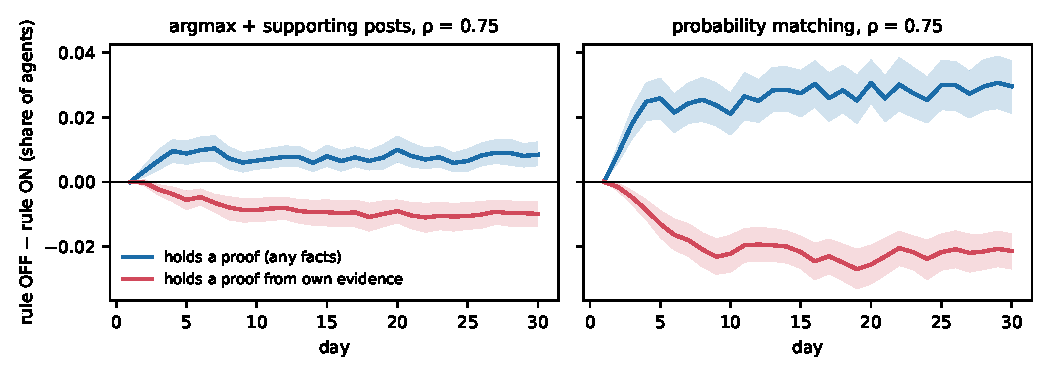
\includegraphics[width=0.95\linewidth]{figures/fig_own_proof.pdf}
\caption{Rule off minus rule on, over days: proof from any facts (blue) and from own
evidence (red). $q = 6$, $q_c = 12$, $b = 1$, $\rho = 0.75$; argmax (left) and probability matching (right).}
\label{fig:ownproof}
\end{figure}

\begin{itemize}\itemsep1pt
\item \textbf{The few extra posts pull the two measures apart} (Figure~\ref{fig:ownproof}):
  more agents hold a proof, but fewer hold one from their own evidence. With the rule on, the truth
  controller already raises the share proving A0 from 28\% to 53\% (day 30, $b = 3$), while the share
  proving it from their own evidence falls to 3\%.
\item \textbf{Mechanism: posting, not reading.} Controller posts are at most 1.5\% of what
  agents read. But an agent passes on one fact a day, and a controller fact it read on
  an earlier day now competes with its original evidence for that slot (Table~\ref{tab:sub}).
  The original evidence circulates less, so fewer agents assemble it into a proof.
  Simulation 2 shows the same substitution.
\end{itemize}

\begin{table}[H]
\centering\small
\caption{What agents read and post, rule on vs off. Truth controller, probability
matching, $\rho = 0.75$, $q = 6$, $q_c = 12$, $b = 3$, all days.}
\label{tab:sub}
\begin{tabular}{lcccc}
\toprule
rule & reads from controller & posts of own evidence & posts of pool facts & own facts held \\
\midrule
on & 1.34\% & 78.3\% & 27.3\% & 5.81 \\
off & 1.50\% & 76.1\% & 29.3\% & 5.67 \\
\bottomrule
\end{tabular}
\end{table}

\section{The controller senses the swarm accurately}

Each night the controller estimates the share of agents backing its target from the
$n \le q_c$ agent posts it reads:
\begin{equation}\label{eq:vhat}
\hat v = \frac{1}{n}\sum_{i=1}^{n} \mathbb{1}\{\text{author of post } i \text{ voted for the target}\},
\end{equation}
and stays silent when $\hat v \ge 0.75$. Each agent posts at most once a day, so the
day's board is nearly a census of votes and $\hat v$ is an unbiased sample of it.

\begin{figure}[H]
\centering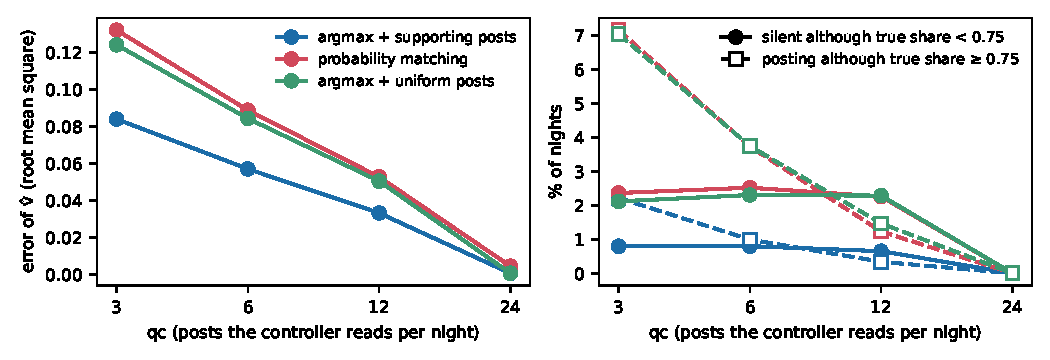
\includegraphics[width=0.95\linewidth]{figures/fig_sensing.pdf}
\caption{Left: error of $\hat v$ against the true share of the 24 agents. Right: gate
mistakes. Mean over arms, $q$, $b$, $\rho$; task003-symmetric.}
\label{fig:sensing}
\end{figure}

\begin{itemize}\itemsep1pt
\item \textbf{No bias}: $\hat v$ minus the true share averages within $\pm 0.0005$ (in Simulation 2 it is
  biased upward).
\item \textbf{The error shrinks with $q_c$} as random sampling predicts, and vanishes at
  $q_c = 24$, where the controller reads every post (Figure~\ref{fig:sensing}, left).
\item \textbf{Gate mistakes are rare} (right panel): under 2\% of nights at $q_c \ge 12$.
  They grow at $q_c = 3$, where the gate needs all 3 posts to agree.
\item \textbf{Abstention does not distort it}: agents almost never abstain (0.1\% of
  agent-days, probability matching only).
\end{itemize}
So in this setup, \textbf{a controller fails because of what it posts, not what it sees.}

%% ---------------------------------------------------------------------------------------------
\section{How readable is the command? Information and pair efficiency}\label{sec:eff}

A controller can change the swarm in two ways: in the direction it is asked to, or in ways that
happen whatever its target. We measure how readable the command is in the swarm (the mutual
information between the target and the swarm's state), which share of the change is directed (the
pair efficiency $\eta$), and how unsure the agents become. Throughout, the target is chosen by a fair
coin, and all quantities are taken at one time $t$, across the 1{,}000 episodes of each arm (not over
whole trajectories). Setting: probability matching, $q = 6$. With full memory every agent proves A0
and nothing is measurable, so only $\rho = 0.75$ is shown.

\subsection{Measures}

\begin{center}
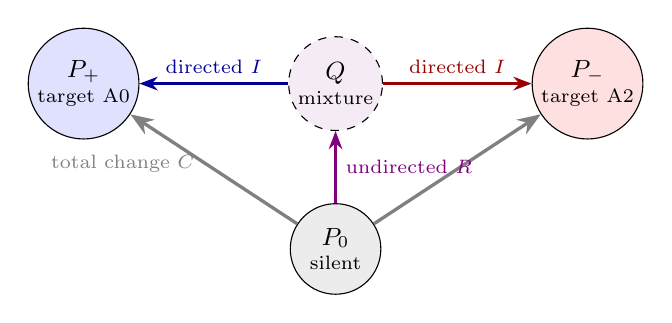
\begin{tikzpicture}[font=\small, dist/.style={draw, circle, minimum size=1.15cm, align=center, inner sep=1pt}]
  \node[dist, fill=gray!15] (P0) at (0,0) {$P_0$\\[-2pt]{\scriptsize silent}};
  \node[dist, fill=blue!12] (Pp) at (-3.2,2.1) {$P_+$\\[-2pt]{\scriptsize target A0}};
  \node[dist, fill=red!12] (Pm) at (3.2,2.1) {$P_-$\\[-2pt]{\scriptsize target A2}};
  \node[dist, dashed, fill=violet!8] (Q) at (0,2.1) {$Q$\\[-2pt]{\scriptsize mixture}};
  \draw[-{Stealth}, very thick, gray] (P0) -- node[left, font=\scriptsize, pos=0.55]{total change $C$} (Pp);
  \draw[-{Stealth}, very thick, gray] (P0) -- (Pm);
  \draw[-{Stealth}, thick, violet] (P0) -- node[right, font=\scriptsize]{undirected $R$} (Q);
  \draw[-{Stealth}, thick, blue!60!black] (Q) -- node[above, font=\scriptsize]{directed $I$} (Pp);
  \draw[-{Stealth}, thick, red!60!black] (Q) -- node[above, font=\scriptsize]{directed $I$} (Pm);
\end{tikzpicture}
\diagramcaption{Three distributions of the swarm's state at time $t$, one per arm, each over the
episodes of that arm. The controller's total change $C$ splits exactly into a part that depends on
its target ($I$, from the mixture $Q$ to each arm) and a part that does not ($R$, from silence to
$Q$). Efficiency $\eta = I/C$ is the directed share.}
\end{center}

\noindent\textbf{Distributions.} For each arm $a$ (silent $0$, target A0 $+$, target A2 $-$) and a
time $t$, each episode $e$ contributes a probability vector $y_a(e)$ over the values $x$ of the
state $X$: at \emph{one-agent} level its vote shares (the vote of a randomly chosen agent), at
\emph{swarm} level a mark on the bin of $s = m_{\text{A0}} - m_{\text{A2}}$ (difference of mean
beliefs, three equal bins on $[-1,1]$). Then $\hat P_a = \frac1n\sum_e y_a(e)$. Any pair of controllers
can be written as
\begin{equation}\label{eq:split}
\hat P_\pm = \hat P_0 + \mu \pm \delta,\qquad \mu = \tfrac12(\hat P_+ + \hat P_-) - \hat P_0,\quad
\delta = \tfrac12(\hat P_+ - \hat P_-),
\end{equation}
a \emph{common} part $\mu$ (what control does on average, whatever the target) and a
\emph{directional} part $\delta$; both are vectors over the values of $X$ (all answers, A1 included).

\noindent\textbf{Readability and the pair efficiency.} With $\hat Q = \hat P_0 + \mu$ and
$\mathrm{KL}(p\Vert q) = \sum_x p(x)\log_2[p(x)/q(x)]$,
\begin{equation}\label{eq:eta}
I = \tfrac12\mathrm{KL}(\hat P_+\Vert\hat Q) + \tfrac12\mathrm{KL}(\hat P_-\Vert\hat Q),\quad
C = \tfrac12\mathrm{KL}(\hat P_+\Vert\hat P_0) + \tfrac12\mathrm{KL}(\hat P_-\Vert\hat P_0) = I + R,\quad
R = \mathrm{KL}(\hat Q\Vert\hat P_0),\quad \eta = I/C .
\end{equation}
$I$ is the mutual information between the target and the state: how readable the command is
(at most 1 bit). With the one-agent state it is $I(\text{target};\text{vote of a randomly chosen
agent})$, the quantity mapped in Figure~\ref{fig:effI}. $I = \frac12\mathrm{KL}(\hat Q+\delta\Vert\hat Q) + \frac12\mathrm{KL}(\hat Q-\delta\Vert\hat Q)$
depends on $\delta$ and on where the pair sits ($\hat Q$); $R = \mathrm{KL}(\hat P_0+\mu\Vert\hat P_0)$ depends
only on $\mu$; $C$ (a number) $= I + R$, so $R = C - I$. The reference $\hat P_0$ is the silent arm. For
small changes, $\mathrm{KL}(p+\epsilon\Vert p) \approx \sum_x \epsilon(x)^2/(2\ln 2\,p(x))$ gives
\begin{equation}\label{eq:etasmall}
I \approx \frac{\Vert\delta\Vert^2}{2\ln 2},\quad R \approx \frac{\Vert\mu\Vert^2}{2\ln 2},\quad
\eta \approx \frac{1}{1 + \Vert \mu\Vert^2/\Vert\delta\Vert^2},\qquad \Vert v\Vert^2 = \sum_x \frac{v(x)^2}{\hat P_0(x)} .
\end{equation}
So $\eta = 1$ exactly when the two controllers' changes are mirror images ($\mu = 0$), whatever their
size, and $\eta$ falls only through the \emph{ratio} of common to directional change: when both push
the same way (a common push), or one moves the swarm much more than the other (a lopsided pair:
along one direction with sizes $a$ and $b$, $\Vert \mu\Vert/\Vert\delta\Vert = |a-b|/(a+b)$). It is a
property of the pair, not of either controller, and it stays constant whenever both effects grow
together; the size of the effect is measured by $I$. At swarm level $C$ is often infinite (the
controlled swarm reaches states silence never visits); there we use $\eta_{JS} = I/(I + \mathrm{JS}(\hat Q,\hat P_0))$ with the bounded
Jensen--Shannon divergence; $\mathrm{JS}(\hat Q,\hat P_0)$ is the information the state carries about
\emph{whether} a controller is present (controlled or silent, 50/50), so $\eta_{JS}$ compares
information about the direction with information about the presence of control.

\noindent\textbf{The agents' own uncertainty}: $\Delta\bar H$ (change in the mean entropy of their
beliefs) and $\Delta$JSD (change in disagreement, the entropy of the mean belief minus $\bar H$),
controlled minus silent, same episode.

\subsection{Over time}

\begin{figure}[!htb]
\centering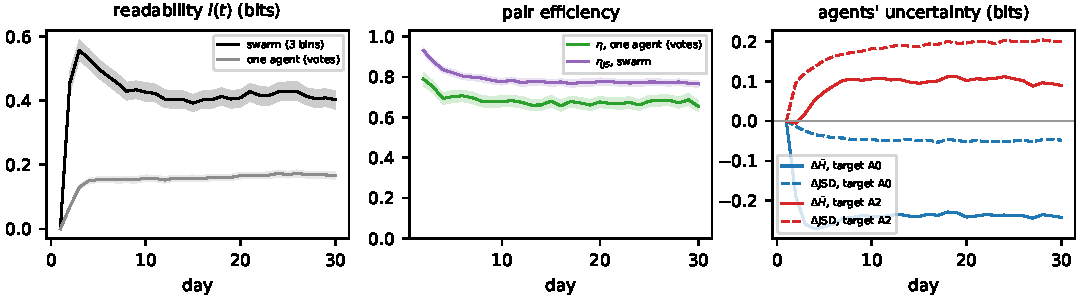
\includegraphics[width=0.92\linewidth]{figures/fig_eff_time2.pdf}
\caption{At $\rho = 0.75$, $q_c = 12$, $b = 3$ (end of each day): readability $I(t)$ at swarm and
one-agent level, pair efficiency ($\eta$, one agent; $\eta_{JS}$, swarm), and the change in the
agents' uncertainty. Bands: 95\% intervals over episodes.}
\label{fig:efftime2}
\end{figure}

\begin{figure}[!htb]
\centering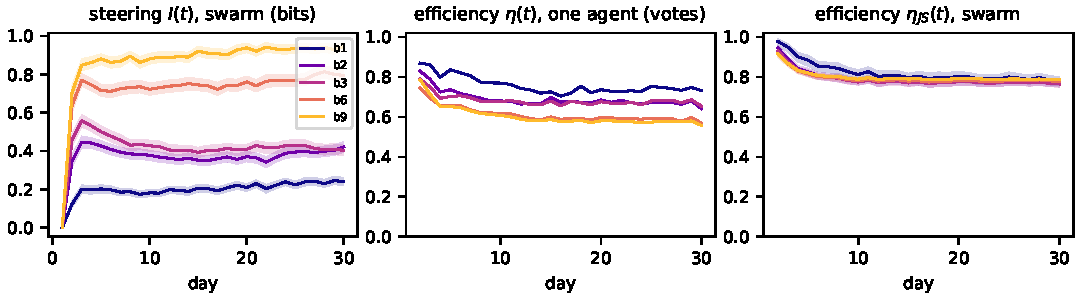
\includegraphics[width=0.66\linewidth]{figures/fig_eff_time.pdf}
\caption{Readability and pair efficiency over the days, $\rho = 0.75$, $q_c = 12$, one line per
facts per night $b$. Bands: 95\% intervals.}
\label{fig:efftime}
\end{figure}

\begin{itemize}\itemsep1pt
\item \textbf{Readability peaks early and settles}: $I = 0.56$ bits (swarm) on day 3, $0.40$ on day 30;
  one agent's vote carries $0.13$ bits on day 3 and $0.17$ on day 30.
\item \textbf{The pair is lopsided} ($\eta = 0.65$, $\eta_{JS} = 0.77$): the false controller moves the
  swarm much more than the truth controller, which is near the ceiling.
\item \textbf{The false controller confuses}: it makes agents less sure ($\Delta\bar H = +0.09$ bits)
  and splits them ($\Delta$JSD $= +0.20$); the truth controller makes them surer ($-0.24$) and more
  alike ($-0.05$).
\end{itemize}

\subsection{Across the control plane}

\begin{figure}[!htb]
\centering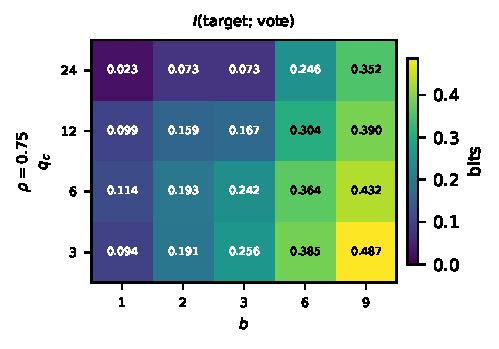
\includegraphics[width=0.36\linewidth]{figures/fig_eff_phase_I.pdf}
\caption{Readability $I(\text{target};\text{vote})$ at day 30, in bits, over the reading budget $q_c$ (y)
and the facts per night $b$ (x); state: the vote of a randomly chosen agent; $\rho = 0.75$.}
\label{fig:effI}
\end{figure}

\begin{figure}[!htb]
\centering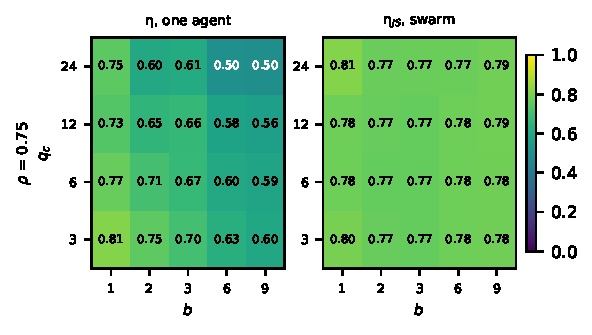
\includegraphics[width=0.32\linewidth]{figures/fig_eff_phase.pdf}
\caption{Pair efficiency at $t = 30$ over $q_c$ and the facts per night $b$: one-agent $\eta$ (beliefs) and swarm
$\eta_{JS}$. Dash: undefined.}
\label{fig:effphase}
\end{figure}

\begin{itemize}\itemsep1pt
\item \textbf{Readability grows with $b$}: from 0.02--0.11 bits at $b = 1$ to 0.35--0.49 at $b = 9$,
  following the false controller's growing gain.
\item \textbf{It falls with $q_c$} (at $b = 9$: 0.49 at $q_c = 3$, 0.35 at $q_c = 24$): reading more
  posts lets the vote gate keep the truth controller silent, so the two targets differ less.
\end{itemize}

\subsection{Readability, pair efficiency and uncertainty against the facts per night}

\begin{figure}[!htb]
\centering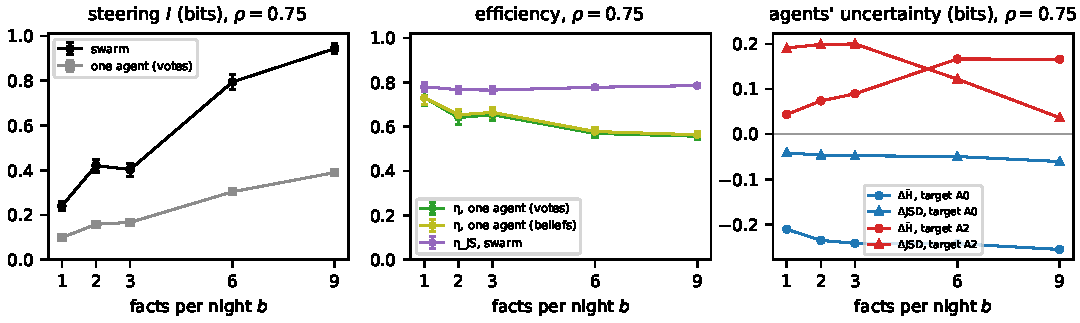
\includegraphics[width=0.72\linewidth]{figures/fig_eff_settings.pdf}
\caption{Readability $I$ (left), pair efficiency (middle) and the change in the agents' uncertainty
(right; circles $\Delta\bar H$, triangles $\Delta$JSD) at $t = 30$ against facts per night $b$ ($q_c = 12$). Bars: 95\% intervals.}
\label{fig:effsettings}
\end{figure}

\begin{itemize}\itemsep1pt
\item \textbf{$\eta$ falls with $b$ (0.73 to 0.56) because the pair becomes lopsided}, not because
  either controller wastes effort: the false controller moves the A0 share from 85\% to 27\% at
  $b = 9$, the truth controller only to 93\% (near the ceiling). On average control then shifts the
  swarm toward A2; that shift is the same whatever the target, so $\eta$ counts it as undirected.
  In Simulation 2 both controllers scale alike and $\eta$ stays at 0.88--0.94.
\item Readability rises with $b$ (swarm 0.24 to 0.94 bits).
\end{itemize}

\subsection{Precision at 50, 100 and 300 paths}

\begin{table}[H]
\centering\small
\caption{Value from 1{,}000 paths per arm, and root-mean-square error of the estimate from 50, 100
or 300 paths (200 random subsets each), at $t = 30$, $b = 3$, $q_c = 12$, $\rho = 0.75$.}
\label{tab:effprec}
\begin{tabular}{lcccc}
\toprule
quantity & 1{,}000 paths & error, 50 & error, 100 & error, 300 \\
\midrule
steering $I$, swarm (3 bins) & 0.403 & 0.059 & 0.042 & 0.023 \\
steering $I$, one agent (votes) & 0.167 & 0.023 & 0.016 & 0.009 \\
efficiency $\eta$, one agent (votes) & 0.655 & 0.063 & 0.044 & 0.022 \\
efficiency $\eta_{JS}$, swarm & 0.765 & 0.038 & 0.029 & 0.012 \\
$\Delta\bar H$, target A0 & -0.242 & 0.031 & 0.020 & 0.010 \\
$\Delta\bar H$, target A2 & 0.089 & 0.035 & 0.024 & 0.012 \\
$\Delta$JSD, target A0 & -0.048 & 0.011 & 0.006 & 0.004 \\
$\Delta$JSD, target A2 & 0.200 & 0.021 & 0.018 & 0.009 \\
\bottomrule
\end{tabular}
\end{table}

\noindent Across all settings, at 100 paths: readability $\pm0.01$ (one agent) to $\pm0.03$ (swarm),
$\eta$ $\pm0.02$--$0.03$, $\Delta\bar H$ $\pm0.02$, $\Delta$JSD $\pm0.006$. Two settings that differ by
at least 0.02 are ordered correctly in 90--100\% of subsets.

%% ---------------------------------------------------------------------------------------------
\section{Success against facts posted}\label{sec:success}

The information measures above say how readable the command is, not whether the swarm ends up
deciding what the controller wants, nor at what cost. Here we measure both directly.

\begin{itemize}\itemsep1pt
\item \textbf{Collective decision} $Y_T$: plurality of the agents' last votes at time $T$; a tie
  between $k$ answers counts $1/k$. \textbf{Success}: $Y_T$ = the controller's target.
\item \textbf{Benefit} $\Delta_\pi = p_\pi - p_0$: change in the probability that the target wins,
  against the silent arm of the same episodes; $p_0$ is the silent probability.
\item \textbf{Cost} $C_\pi$: facts actually posted up to $T$, mean per run (not the allowed budget).
\item \textbf{Best-achievable curve} among the tested settings $\pi$ of one group ($\rho$, target):
  $\Delta^*(B) = \max\{\Delta_\pi : C_\pi \le B\}$, the largest gain reached spending at most $B$;
  read the other way, $C^*(\delta) = \min\{C_\pi : \Delta_\pi \ge \delta\}$, the least spending that
  reaches $\delta$. A setting below the curve is \emph{dominated}: another reached at least as much for less.
\item \textbf{Cost efficiency} $\eta_{\text{cost}} = C^*(\Delta_\pi)/C_\pi$: the share of the spending that
  was necessary (1: nothing cheaper reached as much). Not defined where $\Delta_\pi \le 0$ or its
  95\% interval includes 0.
\end{itemize}

\paragraph{How to read the curves.} Each dot is one setting, at (facts posted, gain). The
\textbf{solid line} is the best-achievable curve over the tested settings: it starts at $(0,0)$ (no
control) and steps up each time a setting reaches a higher gain than anything cheaper; dots on it have
$\eta_{\text{cost}} = 1$, dots below it are dominated, and $\eta_{\text{cost}}$ is how far to the left the
curve reaches the same gain. The \textbf{dashed line} is what becomes reachable if the controller
\emph{chooses its setting at random for each run}: using setting X (7 facts, $+0.32$) in half of the
runs and no control in the other half costs 3.5 facts and gains $+0.16$ \emph{on average}, so every
point on the straight segment between two settings (or between a setting and $(0,0)$) is reachable on
average; the dashed line is the outermost such segments (the concave hull through $(0,0)$). It lies above
the solid line where mixing beats every single setting. Its first segment from $(0,0)$ is arithmetic,
not an observation.

\begin{center}
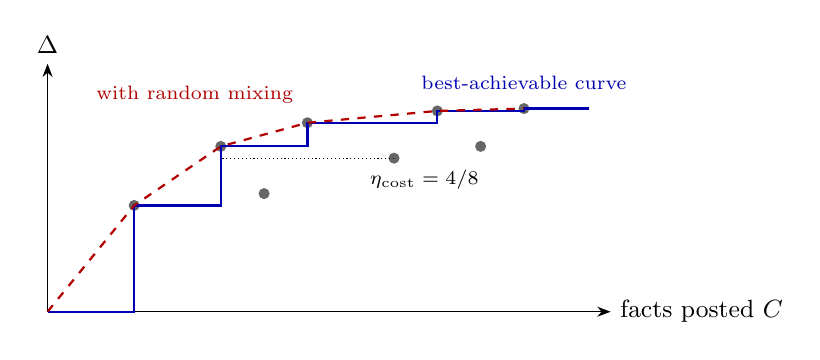
\begin{tikzpicture}[font=\small, x=0.55cm, y=3cm]
  \draw[-{Stealth}] (0,0) -- (13,0) node[right]{facts posted $C$};
  \draw[-{Stealth}] (0,0) -- (0,1.05) node[above]{$\Delta$};
  \foreach \c/\d in {2/0.45, 4/0.7, 6/0.8, 9/0.85, 11/0.86, 5/0.5, 8/0.65, 10/0.7}
     \fill[black!60] (\c,\d) circle (2pt);
  \draw[thick, blue!70!black] (0,0) -- (2,0) -- (2,0.45) -- (4,0.45) -- (4,0.7) -- (6,0.7) -- (6,0.8) -- (9,0.8) -- (9,0.85) -- (11,0.85) -- (11,0.86) -- (12.5,0.86);
  \draw[thick, dashed, red!70!black] (0,0) -- (2,0.45) -- (4,0.7) -- (6,0.8) -- (9,0.85) -- (11,0.86);
  \draw[densely dotted] (8,0.65) -- (4,0.65);
  \node[font=\scriptsize, align=left] at (8.7,0.56) {$\eta_{\text{cost}} = 4/8$};
  \node[font=\scriptsize, blue!70!black] at (11,0.97) {best-achievable curve};
  \node[font=\scriptsize, red!70!black] at (3.4,0.92) {with random mixing};
\end{tikzpicture}
\diagramcaption{Illustration. Each point is a setting. Solid: best-achievable curve; dashed: reachable
on average by random mixing per run. The setting at cost 8 reaches $\Delta = 0.65$, which a setting
costing 4 already reaches: $\eta_{\text{cost}} = 0.5$.}
\end{center}

\begin{figure}[H]
\centering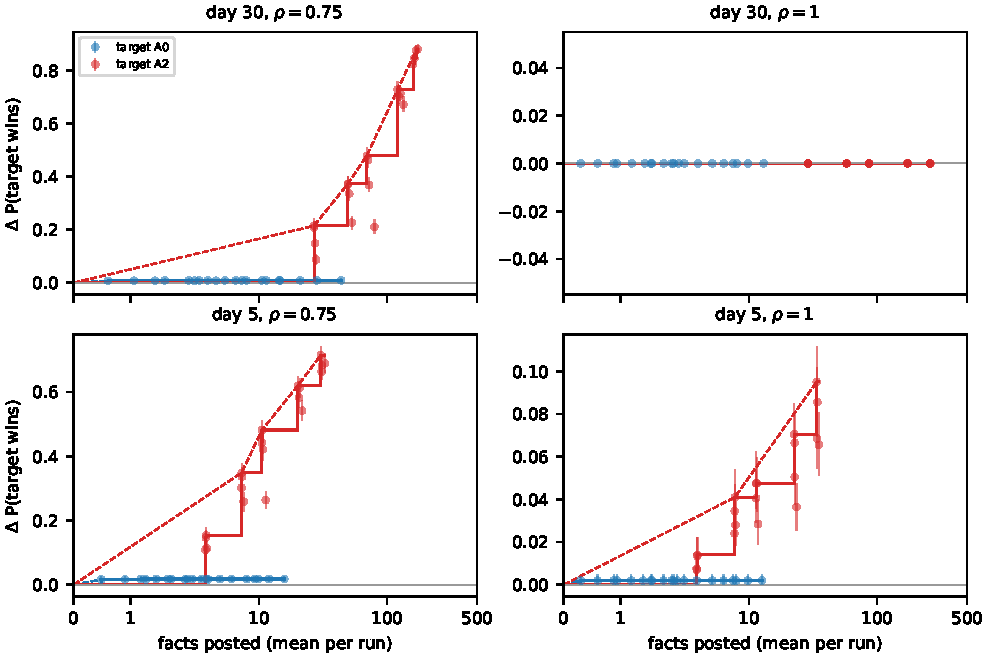
\includegraphics[width=0.84\linewidth]{figures/fig_success_facts.pdf}
\caption{Change in the probability that the controller's target wins against facts posted, on day
30 (top) and day 5 (bottom), $\rho = 0.75$ (left) and $1$ (right); every setting ($q_c \times b$,
$q = 6$, probability matching) with its 95\% interval; blue: target A0, red: target A2. Solid:
best-achievable curve; dashed: with random mixing per run. The x axis is linear from 0 to 1 and
logarithmic above, up to 500.}
\label{fig:success}
\end{figure}

\begin{itemize}\itemsep1pt
\item \textbf{The truth controller has no room}: without control A0 already wins 99.1\% of runs when
  agents forget (100\% with full memory), so its gain is at most $+0.009$ (blue dots near 0).
\item \textbf{Overturning the proof has increasing returns.} On day 30, when agents forget, the false
  controller raises the chance that A2 wins by $+0.09$ to $+0.88$ for 27 to 173 facts, growing faster
  than the facts. The dashed line lies above the solid one: to raise the chance by $0.1$, the best
  single setting needs 27 facts, while mixing a strong setting with no control across runs needs 12.5
  on average ($+0.3$: 49 against 39). Concentrated control pays; the tested settings (a steady batch
  every night) do not include it.
\item \textbf{Here $\eta_{\text{cost}}$ cannot rank the settings}: when the gain keeps growing with
  cost, most settings are the best at their own cost (9 of 20 on the curve, the $b$ ladder; median
  $\eta_{\text{cost}}$ 0.99). That means ``no clear waste'', not ``efficient''.
\item \textbf{With full memory the false controller wins only early}: on day 5 it raises the chance
  that A2 wins by up to $+0.10$ ($b = 9$); by day 30 the gain is 0. When agents forget, the day-5 gain
  already reaches $+0.11$ to $+0.71$ for 4 to 33 facts.
\item \textbf{Precision at 100 paths}: $\Delta$ $\pm0.04$; $\eta_{\text{cost}}$ $\pm0.02$--$0.035$.
\end{itemize}

%% ---------------------------------------------------------------------------------------------
\section{Specific to Simulation 1: other agent rules}\label{sec:rules}

Simulation 2 has only probability-matching agents, so this section has no counterpart there. Simulation 1
also ran \emph{argmax} voting (the most probable allocation) with posts that support the vote (the
\emph{base} rule), and argmax with \emph{uniform} posts (a random remembered fact, whatever the vote).

\begin{table}[H]
\centering\small
\caption{Day-30 paired gain of the false controller in the A2 share, Eq.~(\ref{eq:gain});
$q_c = 12$, $b = 3$.}
\label{tab:rules}
\begin{tabular}{llccc}
\toprule
$\rho$ & agent rule & $q = 3$ & $q = 6$ & $q = 12$ \\
\midrule
0.75 & argmax + supporting posts & 0.95 & 0.85 & 0.26 \\
0.75 & probability matching & 0.48 & 0.32 & 0.08 \\
0.75 & argmax + uniform posts & 0.67 & 0.72 & 0.69 \\
\midrule
1.0 & argmax + supporting posts & 0.03 & 0.01 & 0.00 \\
1.0 & probability matching & 0.00 & 0.00 & 0.00 \\
1.0 & argmax + uniform posts & 0.05 & 0.01 & 0.01 \\
\bottomrule
\end{tabular}
\end{table}

\begin{figure}[H]
\centering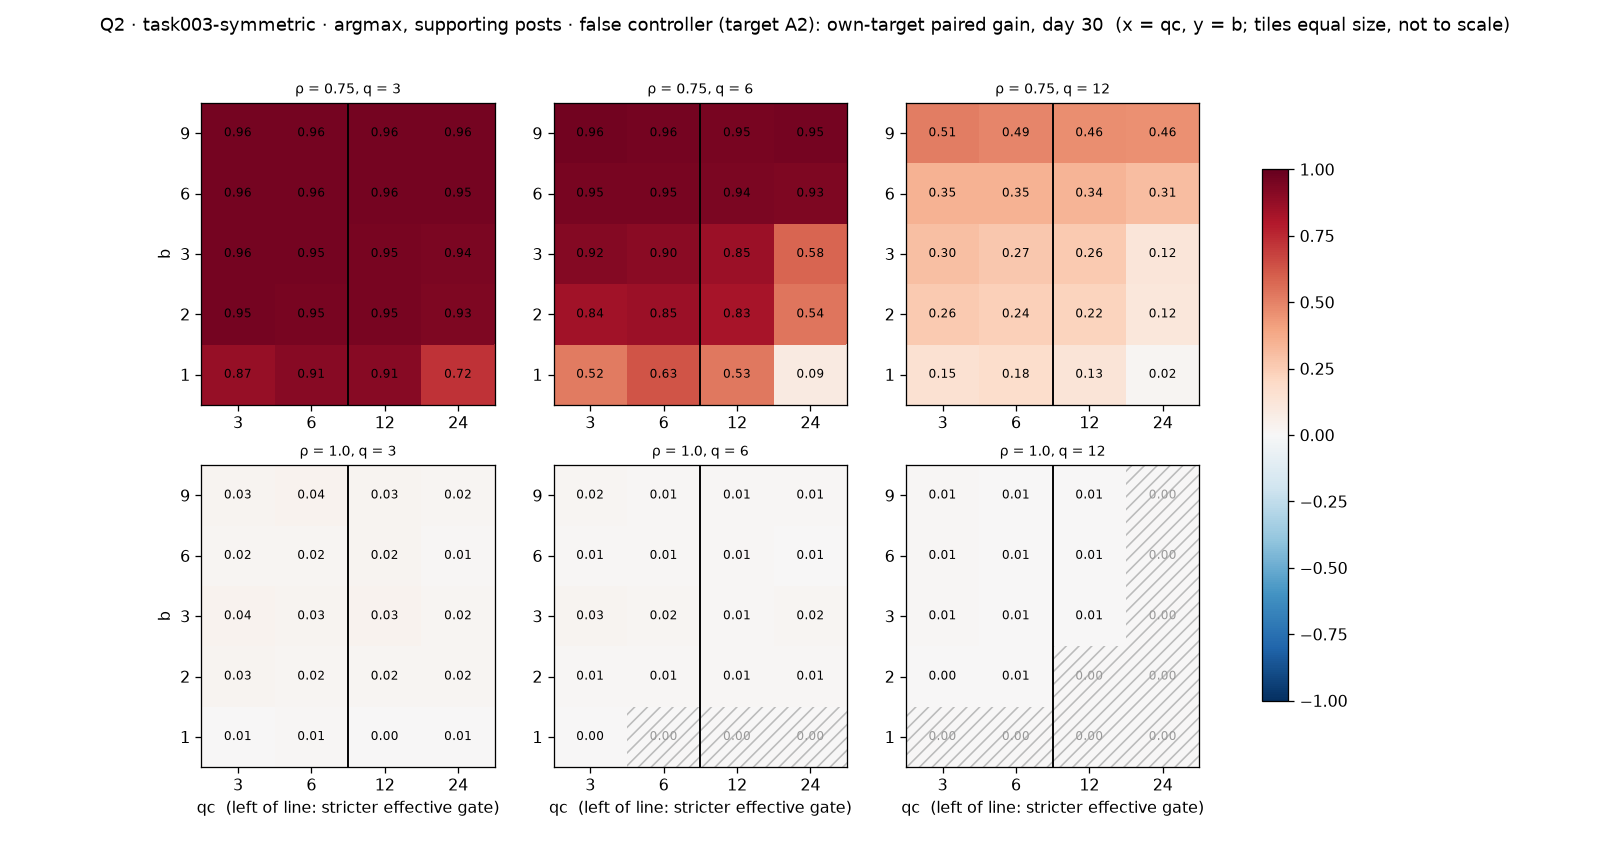
\includegraphics[width=0.92\linewidth]{figures/phase_false_base.png}
\caption{Day-30 paired gain of the false controller (A2 share) over the reading budget
$q_c$ (x) and posting budget $b$ (y); base rule. Rows: $\rho$; columns: $q$. Tiles are
equal size, not to scale. Left of the black line, the vote gate is effectively
stricter (3 of 3, 5 of 6 posts). Note the axes are swapped relative to Figure~\ref{fig:phase}.}
\label{fig:phasebase}
\end{figure}

\begin{itemize}\itemsep1pt
\item \textbf{Argmax makes the false controller much stronger} when agents forget: it pushes the A2
  share from under 0.2 to about 0.9 under the base and uniform rules (gain 0.85 and 0.72 at $q = 6$),
  against 0.32 under probability matching.
\item \textbf{Reading more defends the proof only under supporting posts}: under the base rule the
  gain falls from 0.95 at $q = 3$ to 0.26 at $q = 12$; under uniform posts it stays at 0.67--0.72.
\item \textbf{With full memory every rule ends at A0}: under argmax, 95.6\% of agents hold a proof of
  A0 on day 30 against the false controller, only 42\% from their own evidence.
\end{itemize}

\paragraph{Caveats.} One world (task\_003), 24 agents, exact-Bayesian agents; numbers
are means over 1,000 episodes per cell. Efficiencies are relative to the tested settings. Full
analysis, code and every table: \texttt{analysis/task003\_llm\_free/simulation\_1/analysis/}
(reports Q0--Q6) and \texttt{analysis/task003\_llm\_free/efficiency\_estimates/}.

\end{document}
